\documentclass[10pt]{article}

\usepackage{config/style}

\newcommand{\mytitle}{Object Detection with YOLO}
\newcommand{\myauthor}{
\begin{center}
    Axel H. Grøvdal  \\
\end{center}
}

\title{\mytitle}
\author{\myauthor}
\date{\today}

%----- DOCUMENT -----%
\begin{document}

% Title page
%% Title page
\begin{titlepage}

    \begin{center}
        
        ~\\[1.0cm]
        
        \Large ELE-510 -- Bildebehandling\\[2.5cm]
         
        {\LARGE \textbf{\MakeUppercase{\mytitle}}}
        \vspace{0.5cm}
        \hrule
        
        \vspace{1.0cm}
        \large {\myauthor} 
        \vspace{4.0cm}
        %\vfill
        
        
\includegraphics[scale=0.1]{img/standard_uis.png}
        
        \vspace{0.5cm}
        
        % Bottom of the page
    	{\large \today\par}
        
    \end{center}

\end{titlepage}

% Preface and abstract - edit corresponding file under content/ to change

\pagenumbering{Roman}
\newpage
\section*{Summary}
My task in this rapport were to cover one method of object detection or recognition, write some theory behind it and run some tests. I have chosen to write about the convolutional neural network algorithm You Only Look Once (YOLO) who is one of the fastest object recognition algorithms out in the open marked. It was a bit difficult to decide which algorithm to start with, but after some research, the YOLO algorithm stood out since it was quite fast, open source and therefor popular. 

%YOLO were quite easy to get started with, but had some difficulties with making it work with Python since it is written in C.

% Generates table of contents, list of figures, list of tables
\cleardoublepage % Clear floats
\tableofcontents
\cleardoublepage
\listoffigures
\vspace{1cm}

% Main matter - edit corresponding file under content/ to change
\newpage
\pagenumbering{arabic}
\setcounter{page}{4}
\section{Introduction}

\subsection{Focus area}
This rapport is a project in the subject "ELE-510 Image Processing with Robot Vision". The original task were "Detection of one known object", like a dog, flower, tree etc. However this rapport will focus on recognition of objects using an convolutional neural networks (CNN). This means that recognition of any form of object the neural network is trained to detect, will be tried to be detected. This mean optimally it will not only recognise one single object, but all those object it is designed to recognise. 

\subsection{Object detection and recognition}
Since the focus area of this rapport will be object recognition and not object detection, it is important to know the difference between those two terms. 

\subsubsection*{Object detection}
Object detection, is detecting one certain object given it is in the picture. For a program designed to detect number plates, the input should be an image containing a number plate. Then the output should be a bounding box around the number plate, if it exist. Or it could be the spatial position of the number plate to be used later. Practical use for this type could be an automated toll station who need the number plate of the vehicles driving trough the toll station.

This mean that object detection only can detect what it is supposed to detect.

\begin{figure}%
    \centering
        \subfloat[Object detection]{{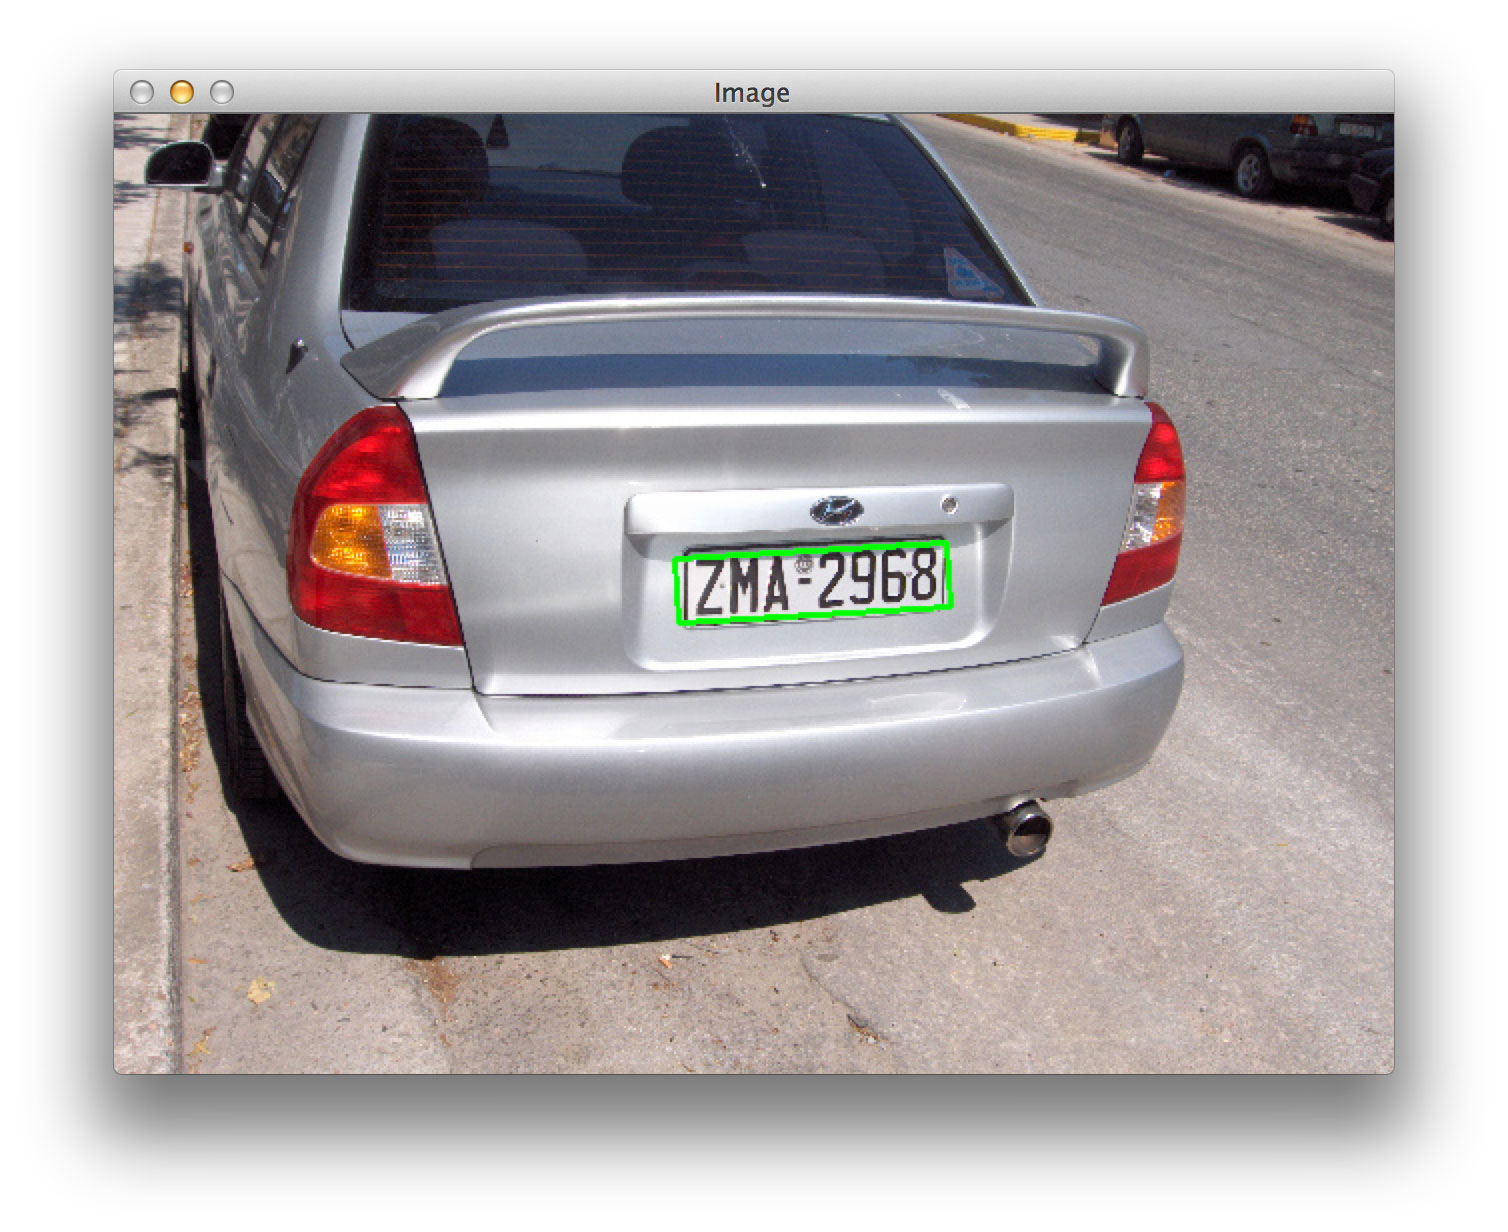
\includegraphics[width=6.5cm]{img/license_detection.jpg} }}
    \qquad
        \subfloat[Object recognition]{{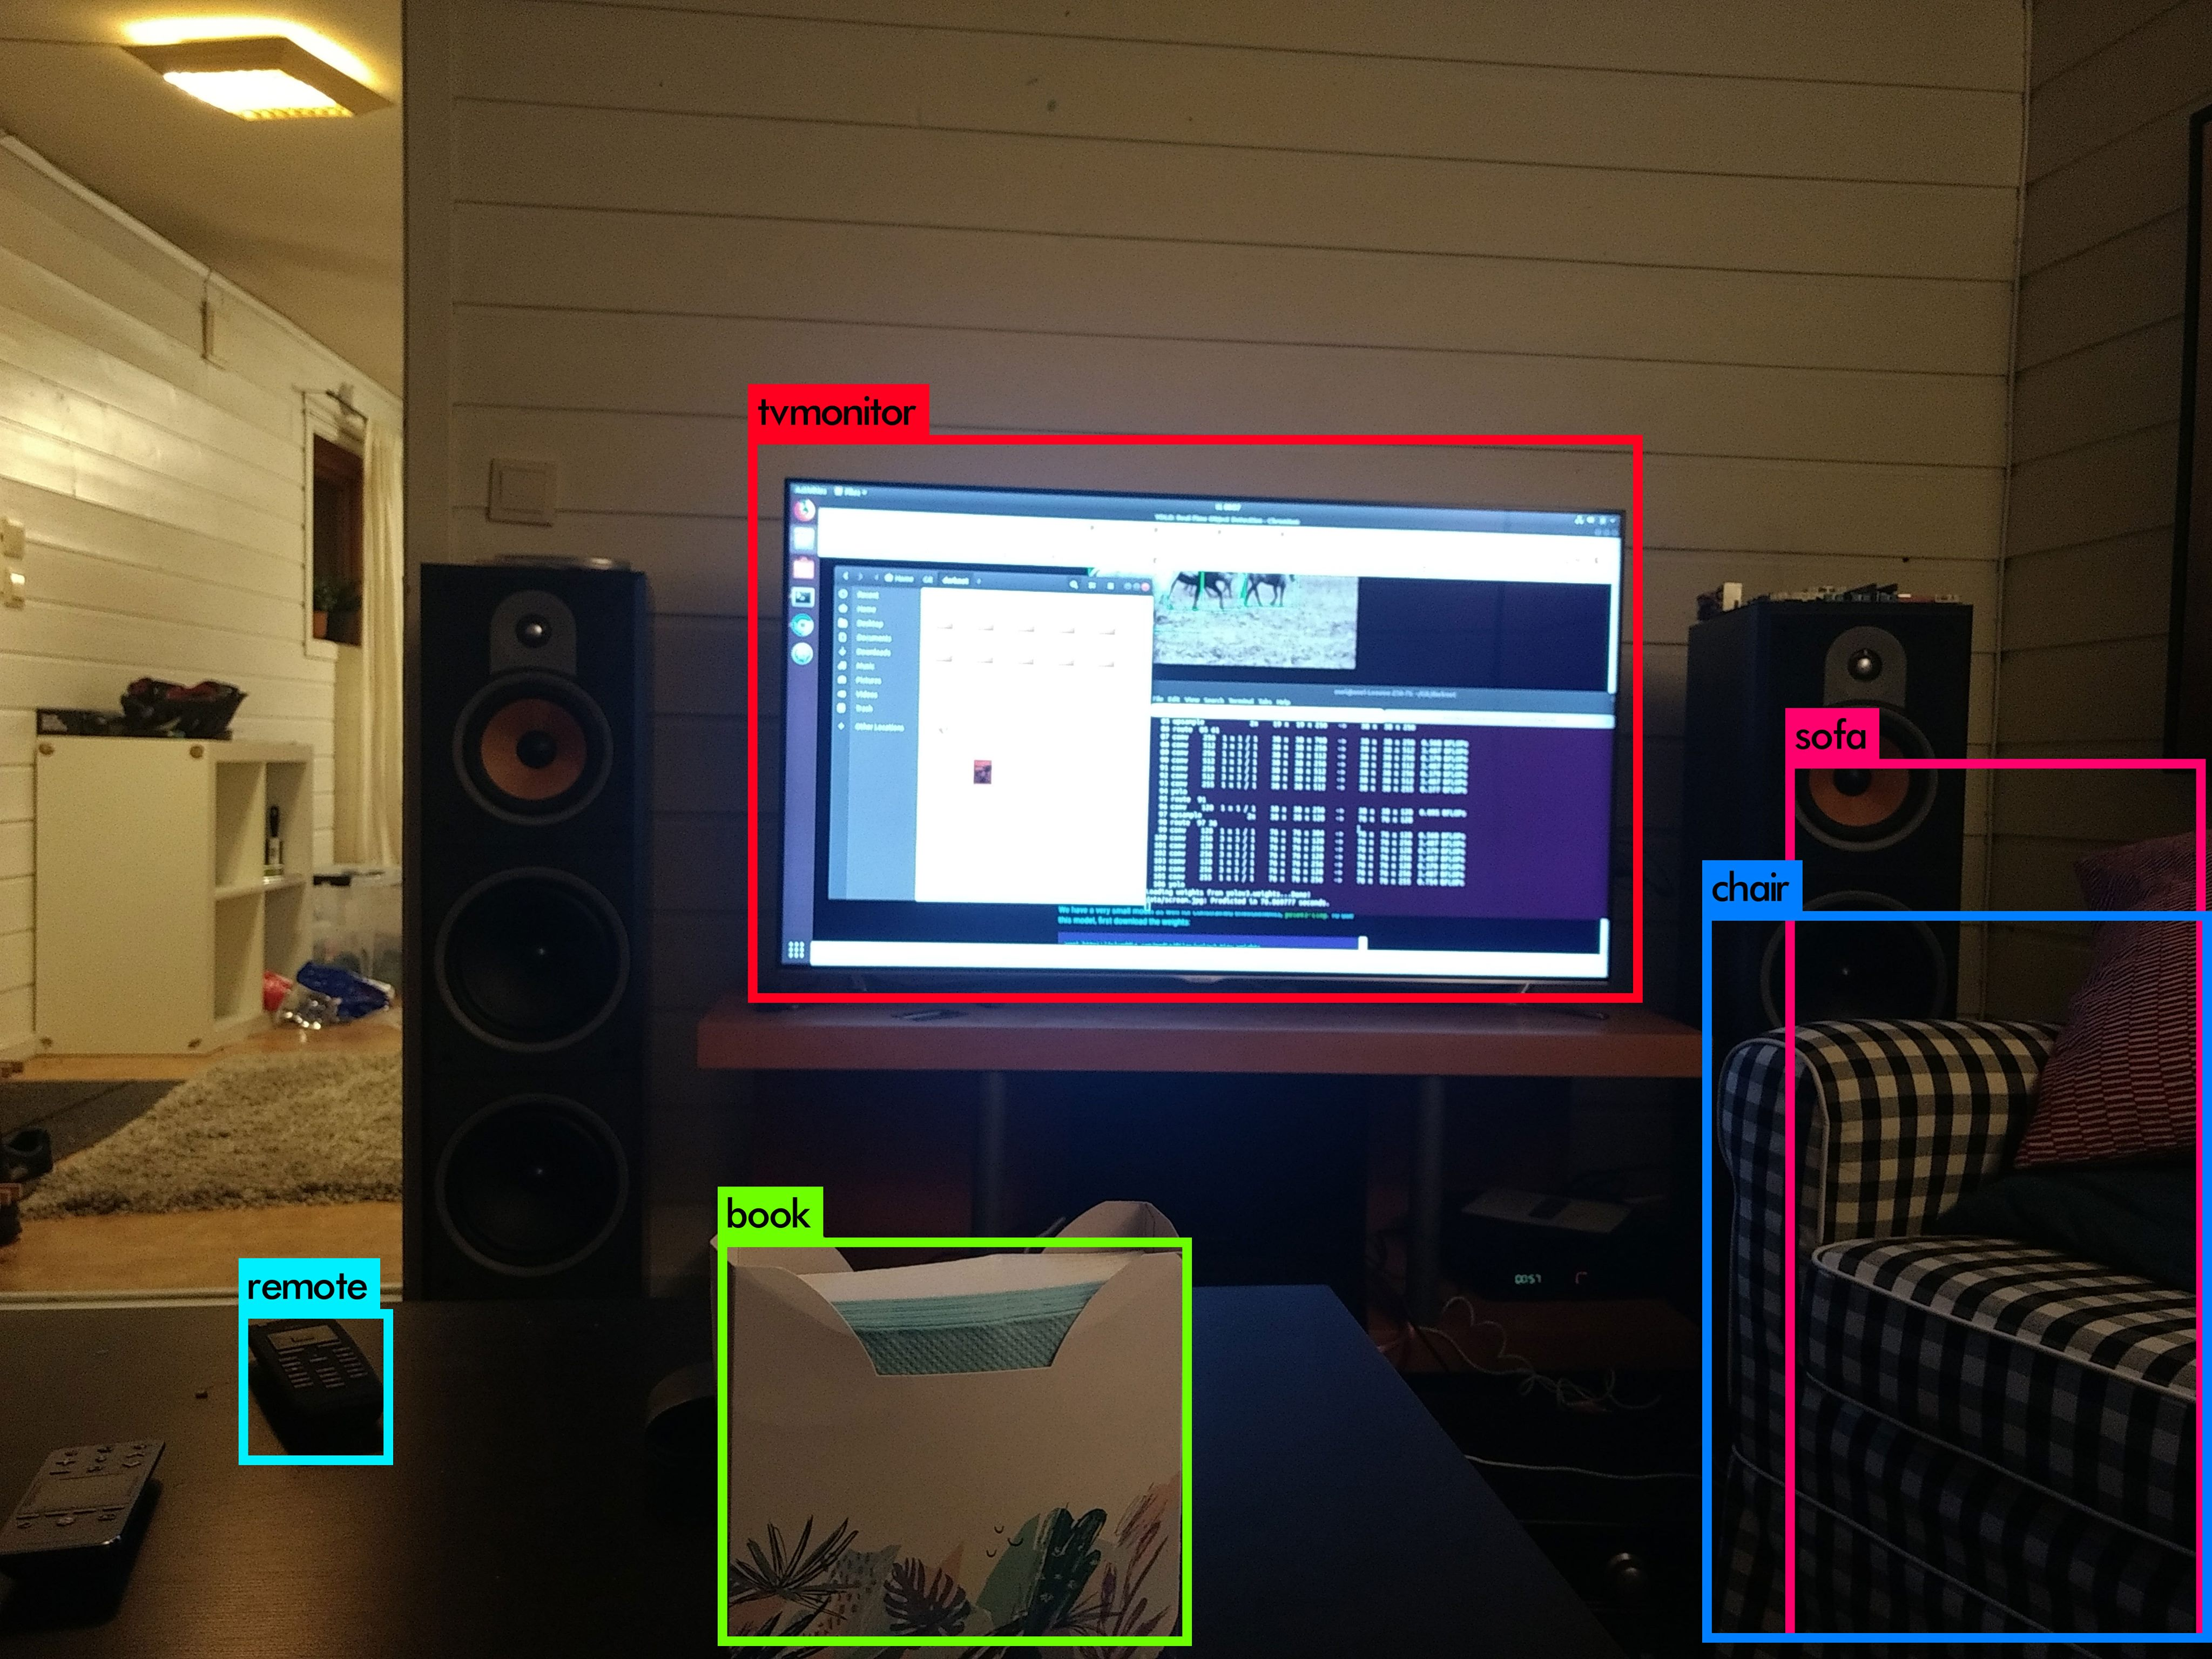
\includegraphics[width=6.5cm]{img/or.jpg} }}
    \caption{Object detection and object recognition}
    \label{fig:OdVsOr}
\end{figure}

\subsubsection*{Object recognition}
Object recognition is recognising different objects in an image or video. A typical input is a video stream or an image, and the output will be bounding boxes around images with a marker telling what the object is. Like for instance, car, bird, person. This mean that object recognition can detect and distinguish what kind of object there is in the sample.

Now there is multiple ways using object recognition, but the widely used methods is by "Machine Learning" or by "Convolutional Neural Networks".

\subsection{ Why YOLO algorithm}
This rapport will focus on the "You Only Look Once" algorithm by now only called YOLO. YOLO is a quite fast and accurate object recognition algorithm utilising CNN to detect objects. This is as fast as 20-220 images per seconds (FPS) on a nvidia Titan X GPU. The variation of fps is due to the use of different weights in the neural networks. In easier terms this means the accuracy can be reduced in change with higher refresh rate. \textit{The high refresh rate of the YOLO make this quite interesting and popular. } \cite{yolo_res}
\newpage

\section{Theory}

This section will be a trivially way of explaining how the YOLO algorithm work. It will also contain explanations of how the different parts of the algorithm works.

\subsection{Convolutional Neural Network}
Convolutional Neural Networks (CNN) is a part of the backbone structure of most object recognition software, as well as YOLO. Therefor it is important to understand how the recognition part of the algorithm works

A CNN consists of an input layer and an output layer. In between there are multiple hidden layers, who is not of any importance, exept the CNN it self. In the hidden layers is where the processings are happening. In the YOLOv1 algorithm, the hidden layers consists of convolutional layers, max pool layers and fully connective layers \cite{YOLO}. Later versions have included other layers as well.\cite{YOLOv3}


\subsubsection{Convolutional layers}
This layer applies learnable convolutional filters to the input data. YOLOv1 utilises as many as 24 convolutional layers. Each layer add their own feature to the image. The convolutions runs spatialy trough the input image. Sliding in height, width and trough the different layers. The convolution net could be divided into 10x10x3 pixels (px). This meaning an image of 100x100x3 px need 100 convolution when going trough one small image. 

The important information that comes from the convolutional filter contains details of the image, how pixels are arrange in spatial and what object is in those pixels \cite{SF_ConvNet}.

\begin{figure}%
    \centering
        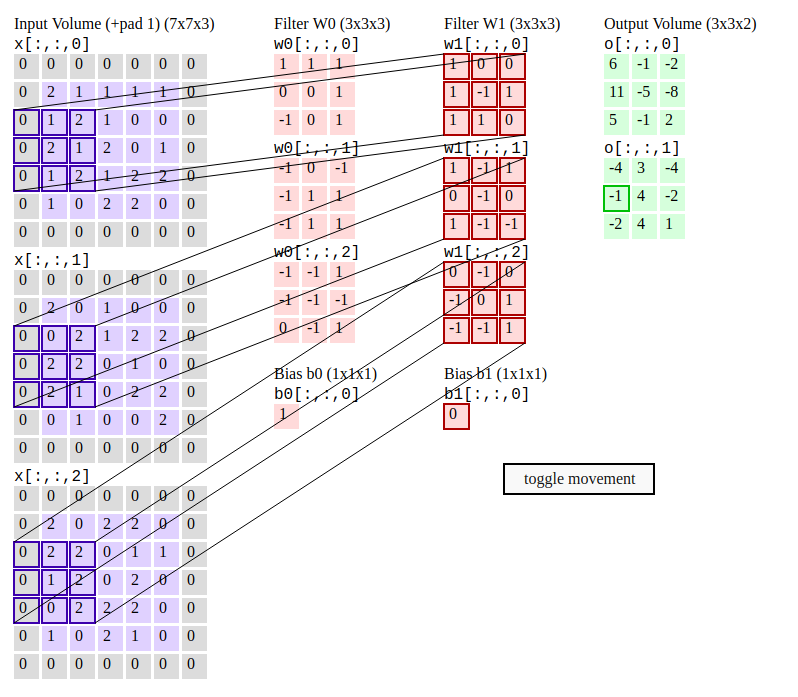
\includegraphics[width=10cm]{img/convNet.png} 
    \caption{Convolutional net with two filters \cite{SF_ConvNet} }
    \label{fig:SF_convNet}
\end{figure}

\subsubsection{Max pool layer}
Used for down-sizing the layers in-between convolutional layers. Max pool layer using the MAX operation to downsample the size, making it smaller and faster to compute the next layers. Normally the max pool filters are size 2x2, and will therefor reduze the pixel count by 75\% after the operation. The depth of the image will be the same. See figure \ref{fig:maxpool} for more information. \cite{SF_ConvNet}
\begin{figure}%
    \centering
        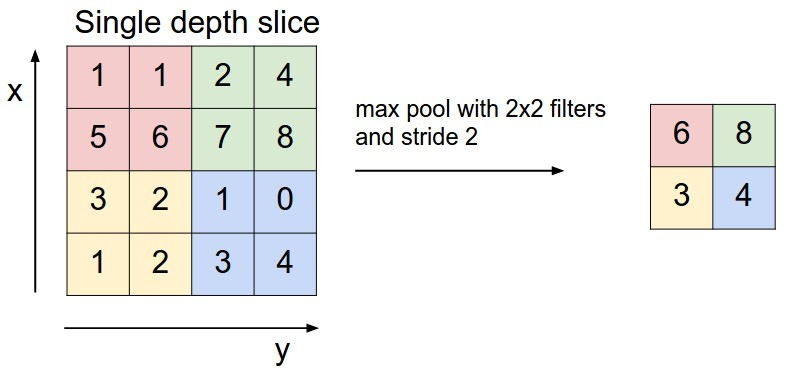
\includegraphics[width=10cm]{img/maxpool.jpeg}
    \caption{Max pool operation \cite{SF_ConvNet} }
    \label{fig:maxpool}
\end{figure}

\subsubsection{Fully Connective layer}
The fully connective layer have connections to all previous layers and is normally at the end of the "hidden layer", right before the output layer. This fully connective layer will calculate the probability of what different object are in specific position in that image with a bias. This is done by looking up highlighted areas produced by matching the highlighted areas from the convolutional filters with an activation map provided by the weight and training. \cite{FCC}

\subsection{Training and Weights}

In order to get the convolutional layers to get their activation map, they need training. The training is done by letting the convolutional neural network process many images, maybe up to tousands of images for each object it should recognise. This recogintion phase is often done by a process called "Backpropogation". The backpropogation is done by feeding the CNN images with tags, so the network will learn to recognise key parts of different objects. A key part could be the ears of a cat. By providing enough of those images the filters will learn how to recognise different key object, who is a known feature to a specific object.

How many training images is needed depends on how well the accuracy is. However a complex weight will also demand more computations, who result in more time to process each image. There is many factors involving in how efficient the object recognition process is, but a proper sized and well trained weight is important.

Often is the weight trained on predefined imagebanks who is available online. For instance some of the YOLO weights who are published, are build on the Common Objects in COntext (COCO), image bank who is available online \cite{darknet13}.

\subsection{Intro to YOLO}\label{yolo_intro}
YOLO is an algorithm who utilises convolution neural networks (CNN) to detect object in image or video. As other approaches on image detecting with CNN like the R-CNN algorithm, they first create potential bounding boxes in the image for then to run a classifier on those boxes. After the classifier has run, post-processing remove the duplicated detections and re-trim the boundingboxes and calculate new probabilities on those boxes. \cite{rcnn}

During the traditional R-CNN algorithm, the image is run trough several times and each different component need to me trained separately. This takes a lot of time and computations. It is quite accurate, but on the cost of time. In the YOLO algorithm it is done by a single regression problem, and create the bounding boxes, probabilities and coordinates directly from the image. In order to do this task, the algorithm only iterate one time trough the image, or "You Only Look Once". The rest of the chapter will go more into details on how it is done.

\subsection{Performance}
Since YOLO only goes trough the image once, it has a potential to be quite fast. In order to utilise the performance, two different steps are essential. During compilation time, YOLO is set to choose where to be processed, GPU or CPU, and witch weight is chosen.

For comparison, a decent CPU uses about 10 seconds to render one image. Using the same weight, a high end consumer GPU have to ability to render 40 frames per seconds. \cite{yolo_res}
\subsubsection*{Hardware - GPU and CPU Rendering}
With the lightest weight and on a Nvidia Titan X GPU, performance can hit about 220 frames per second, or FPS. In order to do so it is necessary to be an Nvidia GPU with CUDA capabilities. A non CUDA GPU is not supported. Why it run so fast and only featured with CUDA is because the framework of "Darknet" the backbone of YOLO is written in CUDA using "TensorFlow". TensorFlow is a framework for creating CNN and Artificial Neural Networks (ANN). The slower option is to use a CPU to process the images. This option is quite slow, but a decent CPU would be able to render an image in about 10 seconds. An older laptop CPU would render one image in about 75 seconds. 

Correct hardware is by other means quite essential for a usable real-time algorithm. 
\subsubsection*{Network Design in YOLOv1}
When the convolutional network was designed, it was designed to pass the Pascal VOC detection dataset as good as possible. The architecture with GoogLeNet model for image classification as inspiration, according to the developer J. Redmon. There are designed two YOLO CNN, a normal one with 24 convolutional layers and 2 fully connected layers and the Fast YOLO. The last one uses only 9 convolutional layers \cite{YOLO}. For more information see figure \ref{fig:yolo_Convnet}.

\begin{figure}
    \centering
        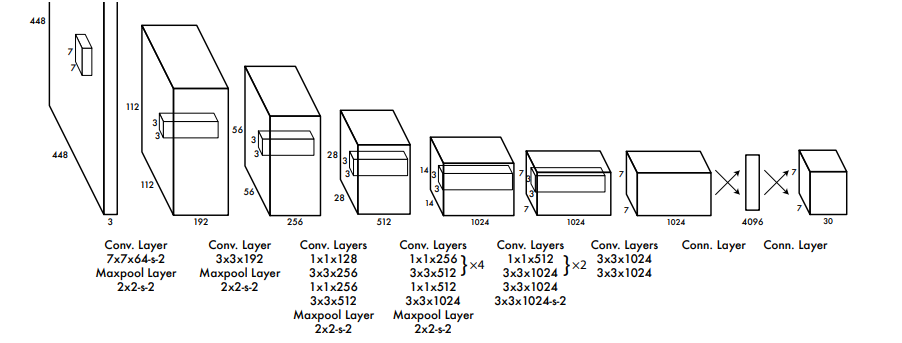
\includegraphics[width=15cm]{img/yolo_CONVnet.png}
    \caption{The CNN architecture used in YOLOv1 \cite{YOLO} }
    \label{fig:yolo_Convnet}
\end{figure}

\subsection{Why is YOLO faster?}
Like mentioned in section \ref{yolo_intro} the YOLO algorithm only look once tough the image. When YOLO take an input image, it resizes the image to for instance 416x416 pixels, and create a grid consisting of 13x13 squares. (The actual pixel size variates in the different versions of YOLO.) In each of those squares YOLO create 5 bounding boxes and calculate the probability of what object is in those bounding boxes \cite{YOLOv2}. After creating the bounding boxes, the boxes probability of containing an object is computed. All boxes giving back a probability parameter below a set threshold value is being discarded. After this process, the bounding boxes covering the same object is being connected, forming one bounding box per object, ideally. 
\newpage

\section{Implementation of YOLO}
To start using YOLO you first need hardware and software who support it. Since my computer does not have a GPU with CUDA cores, this implementation will only cover how to use YOLO with CPU rendering. 

First of all, Darknet, the backbone of YOLO runs nativly in Linux, so that is what I used to implement YOLO. Since YOLO is open-source, other people have made ported version into windows, but this will not be covered.

\subsection{Set up Darknet}

Setting up Darknet is quite straight forward:
\begin{itemize}  
\item Clone git repo
\item Run make inside of Darknet folder
\item Test for errors by launching Darknet trough Terminal.  
\end{itemize}

\lstset{language=Python}
\begin{lstlisting}[frame=single]  
#Download and install Darknet
git clone https://github.com/pjreddie/darknet.git
cd darknet
make

#Test Darknet:
./Darknet
#Output should be:
# "usage: ./darknet <function>"
\end{lstlisting}


\subsection{Get YOLO going}\label{getYOLOgoing}
After downloading Darknet, it is necessary to download the weights and cfg files from web page "pjreddie.com/darknet/yolo/".

Weights can be placed in Darknet rootfolder or in subfolder. Newer git repoes have the cfg files included in "darknet/cfg", otherwise place them also in the Darknet folder.

Test to check if setting up weights went correctly:
\begin{lstlisting}[frame=single]  
#Open terminal in Darknet root folder
./darknet detect cfg/yolov3.cfg yolov3.weights data/dog.jpg
#Object detection will run. Time from 0.03 to 90 secounds.

# End result will look like:
'''
data/dog.jpg: Predicted in 75.021245 seconds.
dog: 99%
truck: 93%
bicycle: 99%
'''
\end{lstlisting}
Note that this Prediction was done on an older laptop CPU, therefor the long processing time. 
Prediction image is now in "darknet/predictions.png".

\subsection{Darknet with Python}
Since running a script make no practical use, is it important to be able to run this algorithm by yourself in your own program.

Natively, this is written in C, so a program in C / C++ have the best efficiency rate. However is it neat to be able to use it in Python. In the repo who was cloned when installing Darknet, was there an almost finished Python example, and also a porting to be able to use the Darknet library, who is written in C. The "C to python" porting was to be found in "darknet/python/darknet.py".

After some trail and error, the "darknet/examples/detector-scipy-opencv.py" was rewritten to work and can be seen in appendix A.

After running the python example, the output will be a matrix in this form:
 \[
 {[ (Object Name_1,P(object_1), (BB_1(X), BB_1(Y),BB_1(width),BB_1(height)),(Object Name_2, ... )  )]}
 \]
 \newpage
 Running the same test image as in the YOLO test, the output variable would be:
\begin{lstlisting}[frame=single]  
 { [
 ('dog', 0.9878906607627869, (224.08419799804688, 380.34490966796875, 184.73121643066406, 305.8154602050781)), 
 ('bicycle', 0.9838747382164001, (346.02569580078125, 282.224609375, 494.97515869140625, 308.0166931152344)), 
 ('truck', 0.9539919495582581, (578.0675048828125, 126.9221420288086, 209.33059692382812, 96.07025146484375))
 ] } 
 \end{lstlisting}

\newpage

\section{Experiments with YOLO}
Looking at YOLO version 3, it has released two different convolutuional network arcitecture, one light and one normal. There is also a few models of the normal architecture, but they only differ in terms of resolutions inside the CNN. They are all trained on the same COCO dataset.

The different models of the YOLOv3, performance-wise differ in case of accuracy and time to compute.

In this example an image of my living room, who is a bit dark, got backlight is chosen as example since it should be a more difficult image to detect objects in.

The test were used on an older laptop CPU. Using the darknet test function as mentioned in chapter \ref{getYOLOgoing}.

\subsection*{YOLOv3-tiny}
The lightest version of YOLOv3.

Frame rate on fast GPU: 220 FPS \cite{yolo_res}.
\begin{lstlisting}[frame=single]
# Running YOLOv3 Tiny with threshold value of 10% 
# Input:
./darknet detect cfg/yolov3-tiny.cfg yolov3-tiny.weights data/stue.jpg -thresh 0.1

#Output
data/stue.jpg: Predicted in 3.294758 seconds.
laptop: 49%
tvmonitor: 73%
sofa: 16%
chair: 18%
\end{lstlisting}

\begin{figure}[h]
    \centering
        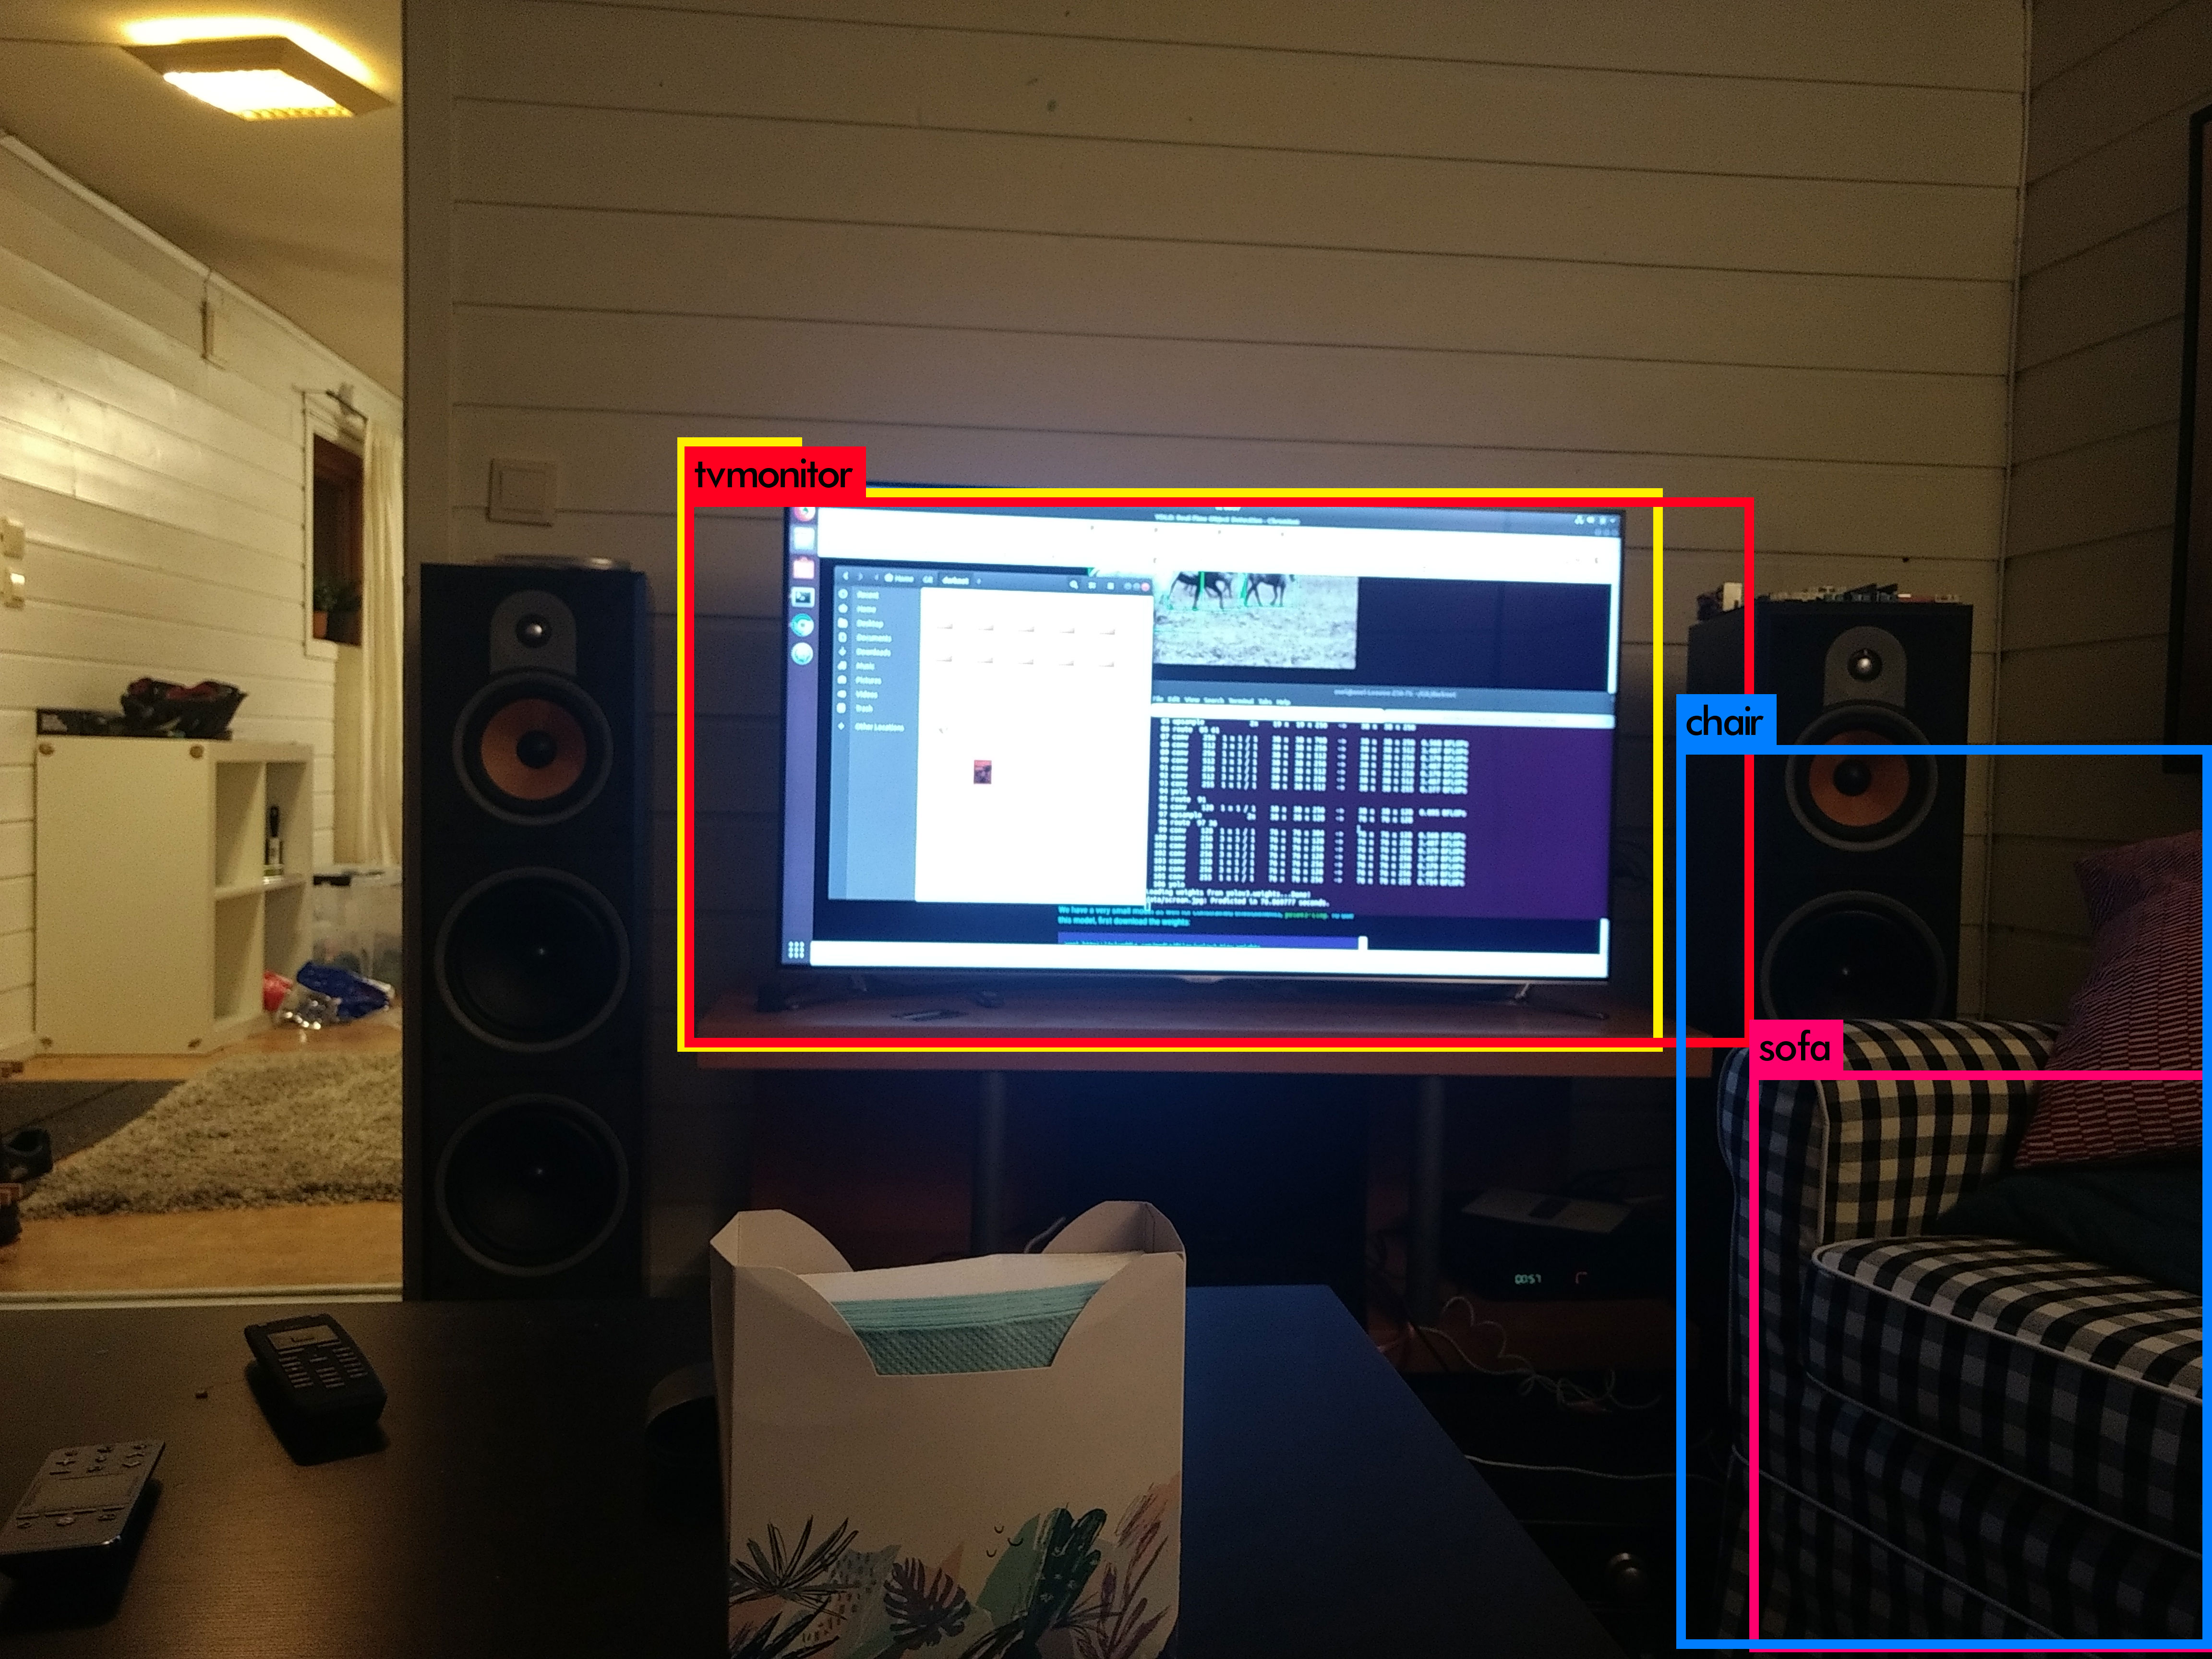
\includegraphics[width=10cm]{experiment_files/YOLOv3_tiny.jpg}
    \caption{Test result form YOLOv3-tiny }
    \label{fig:YOLOv3_tiny}
\end{figure}

\subsection*{YOLOv3-416}
One of the normal versions with a mid range resolution of 416x416.

Frame rate on fast GPU: 35 FPS \cite{yolo_res}.
\begin{lstlisting}[frame=single]
# Running YOLOv3-416 with threshold value of 10\% 
# Input:
 ./darknet detect cfg/yolov3.cfg yolov3_416.weights data/stue.jpg -thresh 0.1
 
#Output
data/stue.jpg: Predicted in 80.764753 seconds.
book: 21%
remote: 31%
tvmonitor: 100%
sofa: 93%
chair: 14%
\end{lstlisting}

\begin{figure}[hb]
    \centering
        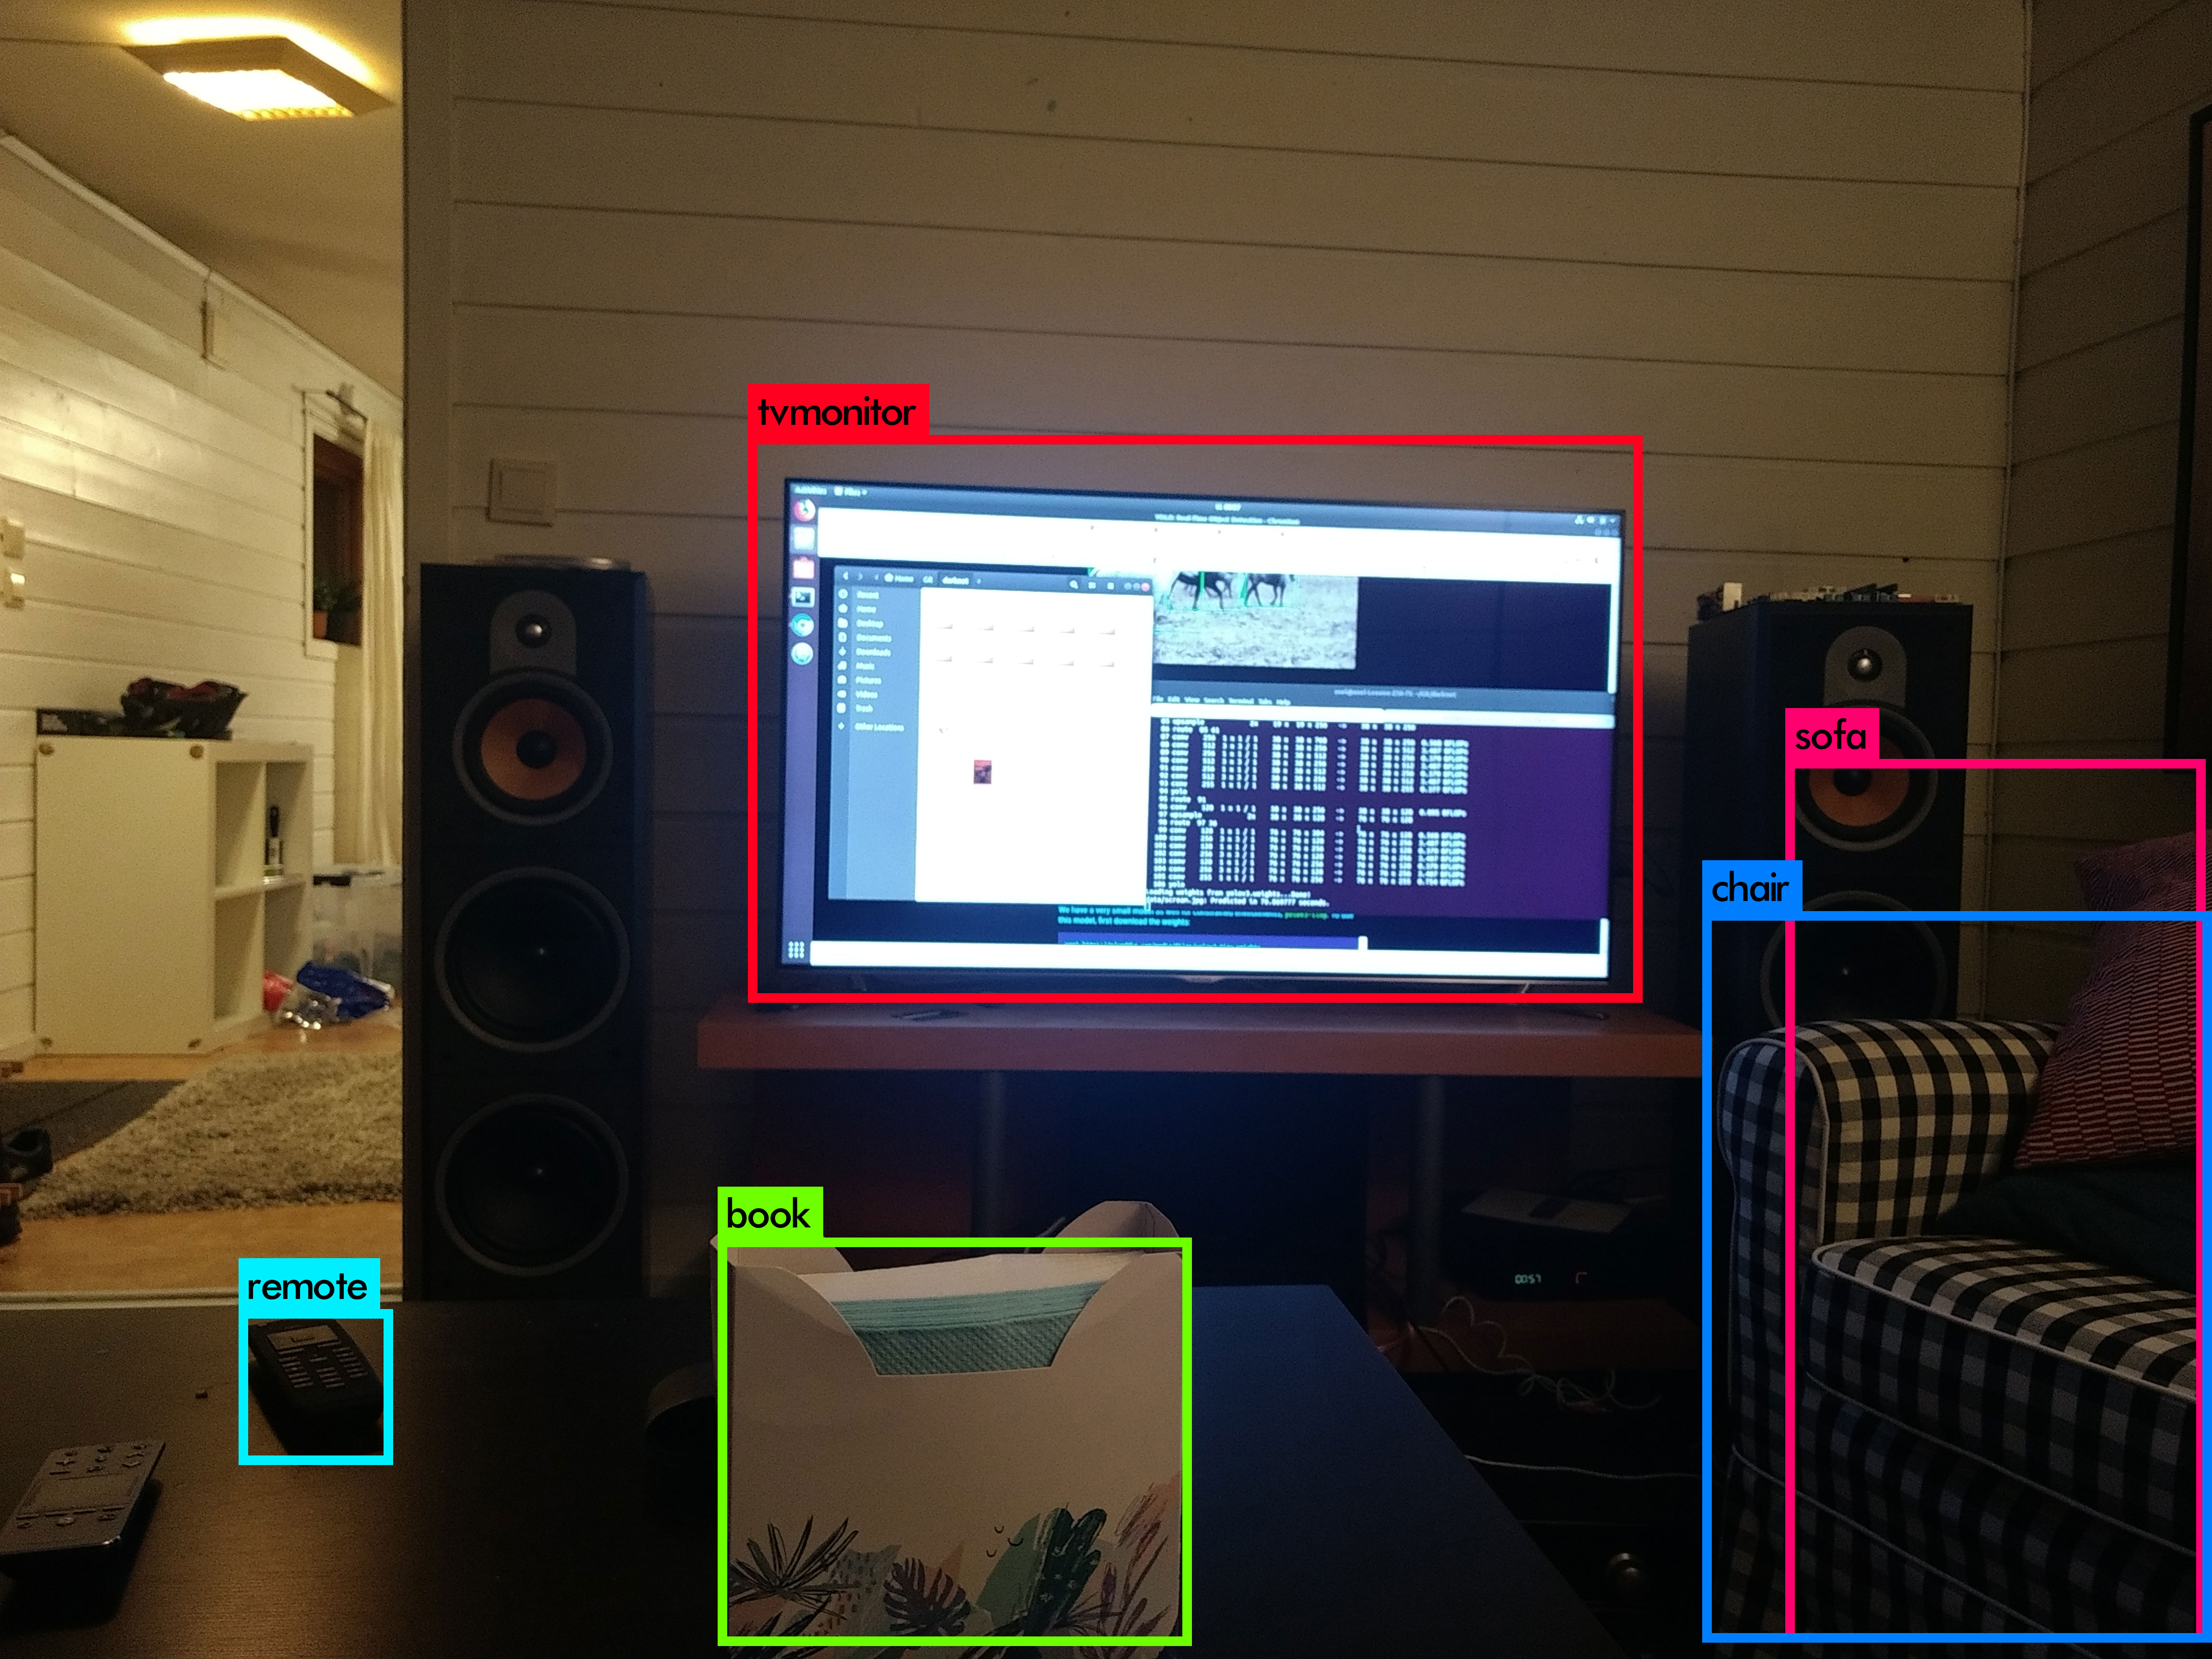
\includegraphics[width=10cm]{experiment_files/YOLOv3_416.jpg}
    \caption{Test result form YOLOv3-416}
    \label{fig:YOLOv3_416}
\end{figure}
\newpage
\subsection*{YOLOv3-spp}
The heaviest version, the YOLOv3-spp

Frame rate on fast GPU: 20 FPS \cite{yolo_res}.
\begin{lstlisting}[frame=single]
# Running YOLOv3_spp with threshold value of 10\% 
# Input:
./darknet detect cfg/yolov3-spp.cfg yolov3-spp.weights data/stue.jpg -thresh 0.1

#Output
data/stue.jpg: Predicted in 78.793520 seconds.
remote: 53%
remote: 43%
tvmonitor: 87%
laptop: 36%
sofa: 93%
\end{lstlisting}

\begin{figure}
    \centering
        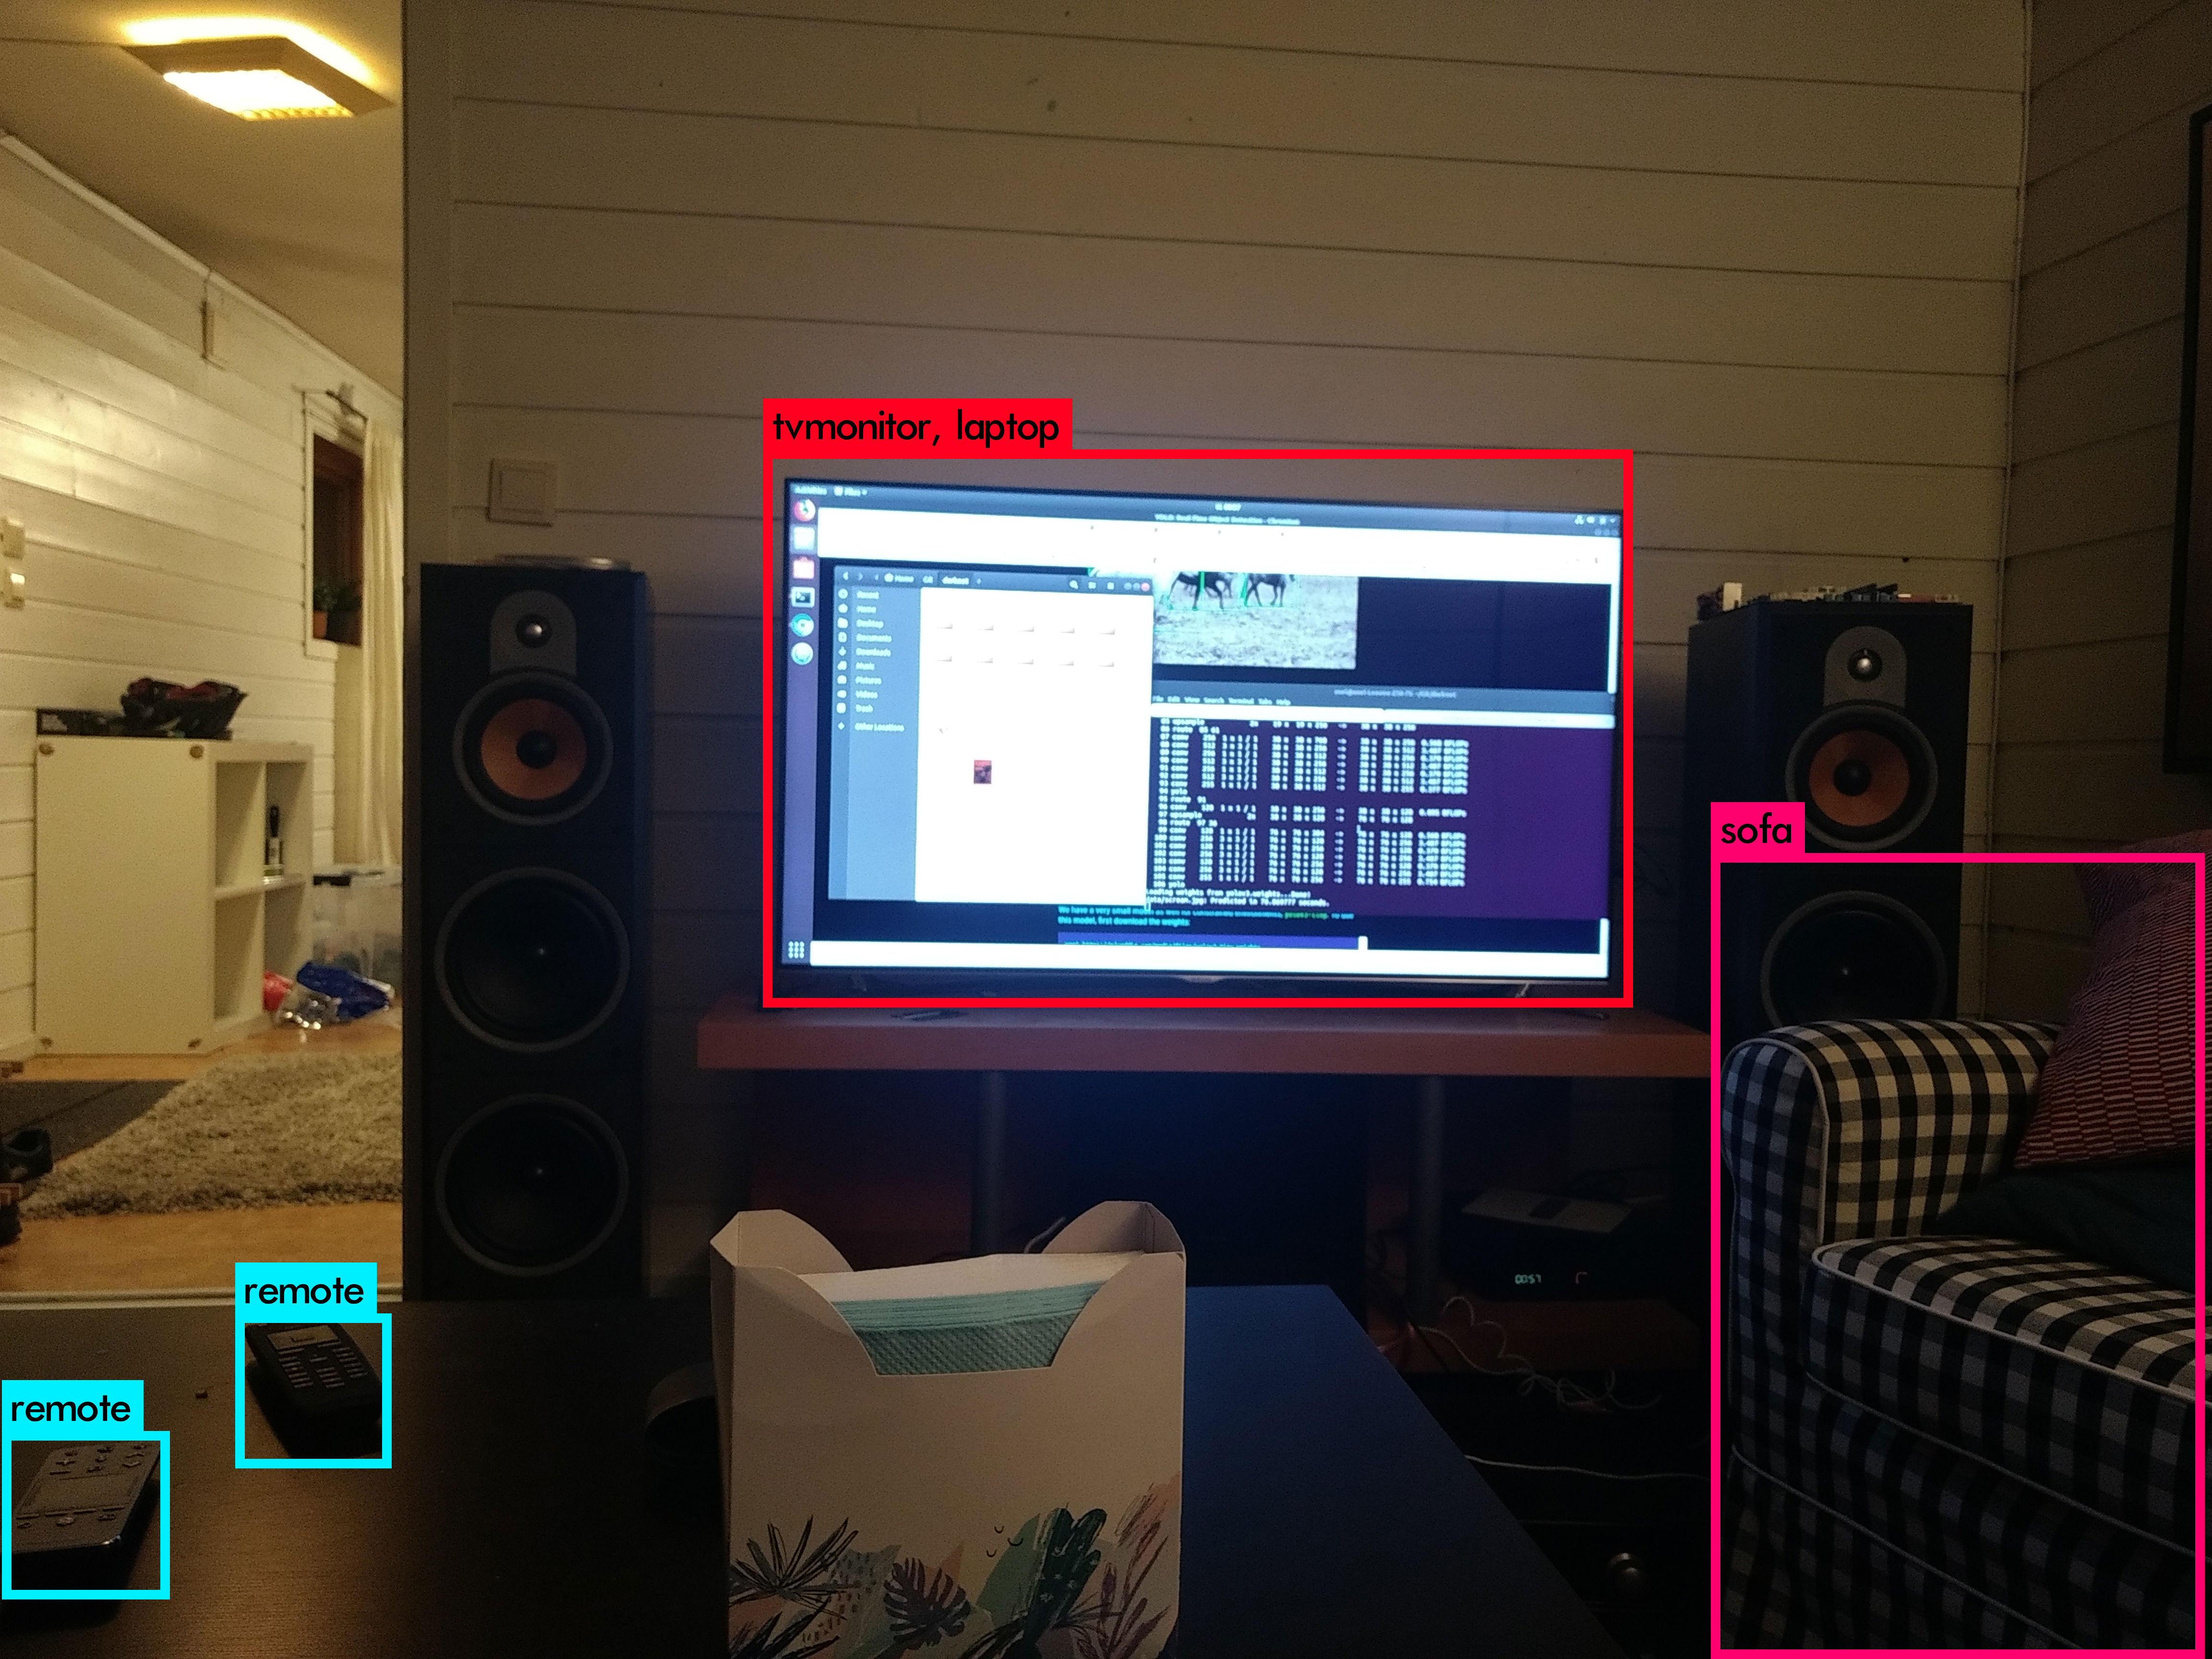
\includegraphics[width=10cm]{experiment_files/yolov3-spp.jpg}
    \caption{Test result form YOLOv3-spp}
    \label{fig:YOLOv3_spp}
\end{figure}

\subsection{Test Results}
After reviewing the test results, did all the different versions find some correct detections and some wrong detections.

\subsubsection*{Performance}
\begin{table}[]
\begin{tabular}{l|lll}
Model       & Test CPU time {[}s{]} & Cited\cite{yolo_res} time from GPU {[}FPS{]} & Cited\cite{yolo_res} mAP-50 score  \\ \hline
YOLOv3-tiny & 3,29                  & 220                           & 33,1               \\
YOLOv3-416  & 80,76                 & 35                            & 55,3               \\
YOLOv3-spp  & 78,79                 & 20                            & 60,3              
\end{tabular}
\caption{My own test result compared to cited performance.}
\end{table}

The test results from the test, shown in table 1 differ performance wise, when comparing the cited GPU time from the tested CPU time for the picture to render. Most remarkable is the speed difference between the normal and the tiny CNN architecture. 3 against 80 second to render an image is quite the big difference. Also the YOLOv3-416 and the YOLOv3-spp had almost the same run time on CPU and on GPU the spp version is roughly 75\% slower then the 416 version. The difference of 2 secunds on the CPU runtime is negotiable, since there is other programs on the computer also using the CPU. The runtime differed between 70-80, when multiple test where run.

However this algorithm is designed as a real time detection algorithm, and test result prove that it is not possible to do real time usage of this algorithm if the test PC does not have a GPU with CUDA cores. But it works fine to do image detection, since run time is not that important.

\subsubsection*{Accuracy}
\begin{table}[]
\begin{tabular}{l|lllllll}
Model \textbackslash Detections {[}\%{]} & TV-monitor & Sofa & Remote 1 & Remote 2 & Book {[}fp{]} & Laptop {[}fp{]} & Chair {[}fp{]} \\ \hline
YOLOv3-tiny                              & 73         & 16   & N/A      & N/A      & N/A                       & 49                          & 18                         \\
YOLOv3-416                               & 100        & 93   & 31       & N/A      & 21                        & N/A                         & 14                         \\
YOLOv3-spp                               & 87         & 93   & 53       & 43       & N/A                       & 36                          & N/A                       
\end{tabular}
\caption{Test results in detecting different objects, including fp (false positives)}
\end{table}
Looking at table 2.
As expected, the tiny version did not perform that well in case of detection accuracy, but it did manage to find the two correct objects, though the confidence score of only 16\% prove it was not certain at all. With a higher threshold, tiny would not detect it at all. 
The YOLOv3-416 and spp, did archived an higher accuracy, but non of them had a 100\% detection rate. The 416 was the only to detect the TV as only a TV, but on all other objects, the spp were quite successfully. 
\newpage

\section{Conclusion}
Convolutional Neural Networks is an technology who make us utilise object detection in an (almost) everyday basis. From smarter search engines, self driving cars, program detecting brain tumours and much more. The YOLO algorithm is one of those algorithm who is not the most accurate, but is one of the fastest, regarding the test computer has a state of the art GPU. YOLO comes as an open source project, making it easy for everyone to modify to suit their own projects. Testing reviled that the YOLOv3-tiny is very fast, but not that accurate, and there is slower alternatives, but still fast, like the YOLOv3-spp who are more accurate. 

% \input{content/0X-conclusion.tex}  %eksempel på div latex triks.

% Bibliography - edit references.bib and use the \cite command in text
\clearpage
\renewcommand{\bibname}{References}
\bibliographystyle{plain}
\bibliography{references}

% Appendices
\appendix
\addappheadtotoc
\newpage
\begin{appendices}
\lstinputlisting[language=Python]{code/hello_darknet.py}
\end{appendices}

% Example text to get started
%\input{example.tex}

\end{document}